\section{Direct calculation}

Consider the broad class of devices that measure the gradient of a scalar field. The idealization is this:
\begin{equation}
  \nabla \phi(x) = \psi(x), \qquad \phi, \psi \in L^{2}.
\end{equation}
The scalar field $\phi(x)3$ is the unknown object of interest and the vector field $\psi(x)$ is the known or measured field. The goal is to invert the equation and solve for $\phi(x)$ in terms of the data $\psi(x)$.

Over each measurement cell or interval of measurement the device registers a value $y_{k}$ corresponding to the average of the gradient of the scalar field over the cell.

Restrict the domain to the real line $\real{1}$, that is the scalar field
\begin{equation}
  \phi: \real{1}\to\real{1}.
\end{equation}
The measurement is the average of the gradient over a finite length,

%%
\subsection[The average of the gradient]{What is the average of the gradient?}
What do the data represent? In other words, what is the average of the gradient over an interval?

Consider the interval $I=[a,b]$ which has length $L=b-a$. The average of the gradient over this interval is defined formally as
\begin{equation}
  \overline{\nabla \phi}_{I} = \frac{\int_{a}^{b}{D_{x}\phi(x)dx}}{b-a}
\end{equation}
where $D_{x}$ represents the total differential operator in the $x$ variable. Using the Fundamental Theorem of Calculus\index{Fundamental Theorem of Calculus} this result is given by
\begin{equation}
  \overline{\nabla \phi}_{I} = \frac{\phi(b)-\phi(a)}{L}.
\end{equation}
The interpretation is basic: if we have knowledge of the average gradient across an interval we know about the \textit{difference} between the end points of the interval. Because we measure a derivative, we can only talk about differences between boundary points. For example the functions $\phi(x)$ and $\phi(x)+\alpha$ where $\alpha$ is an arbitrary constant, both have the same gradient and the same average gradient. That is
\begin{equation}
  \nabla \phi(x) = \nabla \paren{\phi(x)+\alpha}.
  \label{eq:gradient:invariance}
\end{equation}
This invariance will show up in the linear system as a rank deficiency.

There is even a broader class of equivalence. Since the average of the gradient just tells us about the difference between endpoint values, all functions which connect the endpoints are equivalent. An example is shown below. In each case the average of the gradient is zero.
\begin{figure}[htbp] %  figure placement: here, top, bottom, or page
   \centering
   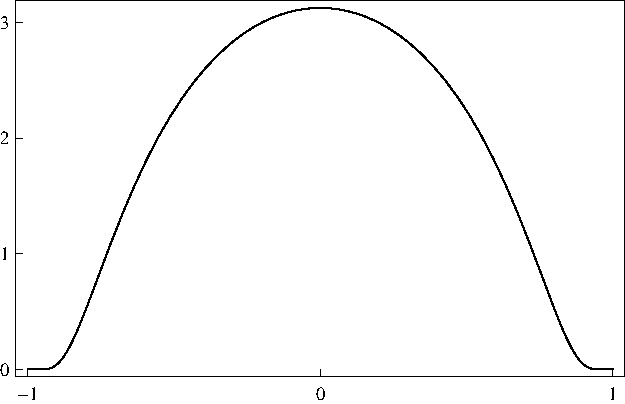
\includegraphics[ width = 1.5in ]{pdf/gradient/gradient_1} \quad
   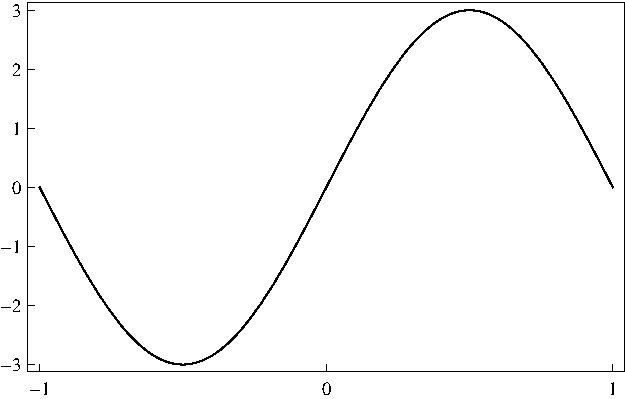
\includegraphics[ width = 1.5in ]{pdf/gradient/gradient_2} \quad
   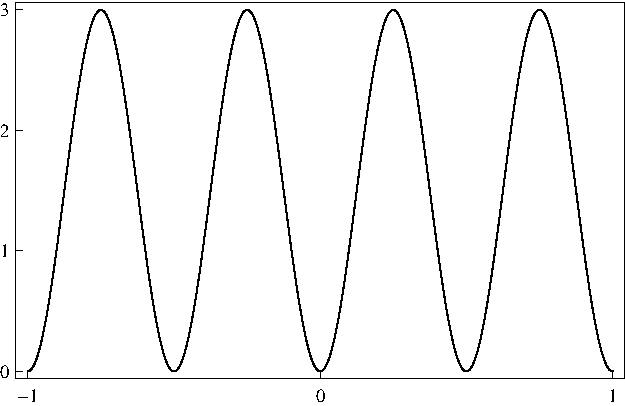
\includegraphics[ width = 1.5in ]{pdf/gradient/gradient_3} 
   \caption{All three of the functions have the same average gradient since the boundary points have the same values. From a mathematical perspective, these functions are indistinguisable under the average gradient operator.}
   \label{fig:gradient:tres}
\end{figure}

Finally, it is convenient to work in cell space\index{cell space} where the length of each cell is identically one. In this case the average gradient over the $k$th cell becomes
\begin{equation}
  \overline{\nabla \phi}_{I_{k}} = \phi(k)-\phi(k-1) = \phi_{k} - \phi_{k-1}.
\end{equation}
Here the function arguments are replaced with integer subscripts tagging the $x$ location of the measurement. For example $\phi(0)$ becomes $\phi_{0}$.

%%
\section{Regularization}
The ambiguity expressed in equation \eqref{eq:gradient:invariance} reveals that we can't solve these problems directly. Just as in the first chapter the general solution has a nontrivial nullspace contribution. One way to think of the issue is to realize that we can't solve for $\Phi$, the values of the fields, instead we can only solve for differences between the field values.

Yet as in the first chapter, we can in fact compute a point solution; we can find a particular solution.  In this section we will regularize the linear system and create a problem with a direct solution. To do this we will introduce another constraint; in essence we will change the problem that we are solving. However, this will not change the particular solution.

We can learn a great deal by starting the simplest systems.  The single cell system demonstrates how the rank deficient system is solved by introducing another constraint. The double cell system which follows demonstrates how the need to arbitrate the vertices which are shared by two cells.

%%
\subsection{Single measurement cell}
Consider the simplest system: a single cell. There are two vertices, the endpoints on the left and right. The left vertex is at $x=0$ and the right vertex is at $x=1$. The cell spans the region between the vertices. The function values will be computed at the vertices and denoted by $\phi_{0}$ and $\phi_{1}$.

A convenient artifice is to represent the function values as sticks as shown in figure ???. We see the scalar field $\phi(x)$ over the sampling area of the cell. The actual field values are shown as $\phi_{0}$ and $\phi_{1}$. However the ideal device measures the average of the gradient which is the height difference $z_{1}$ between the $\phi_{0}$ and $\phi_{1}$. Mathematically the 
\begin{equation}
  \overline{\nabla\phi}_{I_{1}}=z_{1}=\phi_{1}-\phi_{0}.
\end{equation}
Notice that we are solving an idealization where we use the values of scalar field to describe the date. In an experiment the $z$ variables represent the measurements and the goal is to find the field values.

So given a measurement value of $z_{1}$ we only know that $\phi_{0}$ is $z_{1}$ units larger that $\phi_{1}$. What values do we assign to the field values then? The ambiguity takes this form
\begin{equation}
  \paren{\phi_{1}+\alpha}-\paren{\phi_{0}+\alpha}=z_{1}.
\end{equation}
In terms of a linear system we have this
\begin{equation}
  \begin{split}
    \A{}\Phi&=b\\
    \mat{cc}{-1&1}\mat{c}{\phi_{0}\\\phi_{1}}&=\brac{z_{1}}
    \label{eq:gradient:1d:system}
  \end{split}
\end{equation}
which does not offer a unique solution. There is a continuum of field values for the vertices of the form
\begin{equation}
  \phi_{1}=\phi_{0}+z_{1}.
\end{equation}
When we look at equation \eqref{eq:gradient:invariance} we see that the variable $\phi_{0}$ plays the role of the arbitrary constant $\alpha$.

How can we select a single solution? One may choose to fix the constant $\phi_{0} = 0.$ While this will work, this strategy does not extended to two and higher dimensions. Because devices of interest work in two and higher dimensions, we want to avoid this artifice.

To collapse the null space, we need another condition. A useful and natural choice is the \textit{zero sum condition}\index{zero sum condition}:
\begin{equation}
  \sum_{k=0}^{n}\phi_{k} = 0.
\end{equation}
In other words, just enforce the condition that the sum of the field measurements be zero.

With this condition we now have two equations with two unknowns:
\begin{equation}
  \begin{split}
    \phi_{0} + \phi_{1} &= 0.\\
    \phi_{1} - \phi_{0} &= z_{1}.
  \end{split}
\end{equation}
The linear system is then
\begin{equation}
  \begin{split}
    \A{} \Phi &= b\\
    \mat{rr}{1&1\\-1&1}\mat{c}{\phi_{0}\\\phi_{1}}&=\mat{c}{0\\z_{1}}.
  \end{split}
\end{equation}
The solution is given by this
\begin{equation}
  \begin{split}
    \Phi&=\A{-1}b\\
     \mat{c}{\phi_{0}\\\phi_{1}}&=\frac{1}{2}\mat{rr}{1&-1\\1&1}\mat{c}{0\\z_{1}}\\
     &=\frac{1}{2}\mat{r}{-z_{1}\\z_{1}}.
  \end{split}
  \label{eq:gradient:onecell:regular}
\end{equation}
The zero sum condition is manifest:
\begin{equation}
  \phi_{0}+\phi_{1}=-\frac{z_{1}}{2}+\frac{z_{1}}{2} = 0.
\end{equation}
Figure \eqref{fig:gradient:beforeafter} shows depictions of the incident scalar field on the left and the computation on the right. The solutions are equivalent modulo an additive constant.
\begin{figure}[htbp] %  figure placement: here, top, bottom, or page
   \centering
   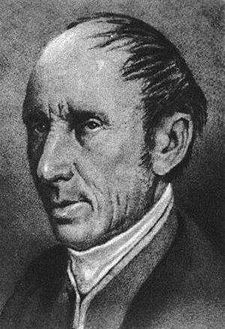
\includegraphics[ width = 1in ]{pdf/gradient/Cauchy.jpg} 
   \caption{Before and after. The physical problem is on the left; the result of the computation is shown on the right.}
   \label{fig:gradient:beforeafter}
\end{figure}

%%
\subsection{Two measurement cells}
Consider the next simplest system: two cells sharing a vertex. The equations are these:
\begin{equation}
  \begin{split}
    \phi_{1}-\phi_{0}&=z_{1},\\
    \phi_{2}-\phi_{1}&=z_{2}.\\
  \end{split}
\end{equation}
The new wrinkle is that the shared vertex $\phi_{1}$ must satisfy two conditions. This represents the usual situation where we use a least squares fit to arbitrate these conflicting conditions.

We again have a rank deficient system reflecting the fact that we have two equations and three unknowns. The linear system is given by this:
\begin{equation}
  \begin{split}
    \A{}\Phi&=b,\\
    \mat{rrr}{-1&1&0\\0&-1&1}\mat{c}{\phi_{0}\\\phi_{1}\\\phi_{2}}&=\mat{c}{z_{1}\\z_{2}}.
  \end{split}
  \label{gradient:2:rd}
\end{equation}

Of course this system has a least squares solution. But before we turn to that in the next section, let's solve this problem by introducing the zero sum condition in the guise
\begin{equation}
  \phi_{0} + \phi_{1} + \phi_{2} = 0.
\end{equation}
Including this constraint with equation \eqref{gradient:2:rd} yields this
\begin{equation}
  \begin{split}
    \tilde{\A{}}\Phi&=b,\\
    \mat{rrr}{-1&1&0\\0&-1&1\\1&1&1}\mat{c}{\phi_{0}\\\phi_{1}\\\phi_{2}}&=\mat{c}{z_{1}\\z_{2}\\0}
  \end{split}
  \label{gradient:2:fr}
\end{equation}
which may be solved by elementary means. The solution is this
\begin{equation}
  \begin{split}
    \Phi &= \tilde{\mathbf{A}}^{-1}b\\
      \mat{c}{\phi_{0}\\\phi_{1}\\\phi_{2}}&=\frac{1}{3}\mat{rrr}{-2&-1&1\\1&-1&1\\1&2&1}\mat{c}{z_{1}\\z_{2}\\0}\\
      &= \frac{1}{3}\mat{r}{-2z_{1}-z_{2}\\z_{1}-z_{2}\\z_{1}+2z_{2}}.
  \end{split}
  \label{eq:gradient:2:reg}
\end{equation}

%%
\section{The least squares solution}
The pseudoinverse will have a new interpretation here.

%%
\subsection{Single measurement cell}
The system was described in equation \eqref{eq:gradient:1d:system}:
\begin{equation*}
  \begin{split}
    \A{}\Phi&=b\\
    \mat{cc}{-1&1}\mat{c}{\phi_{0}\\\phi_{1}}&=\brac{z_{1}}
  \end{split}
\end{equation*}

We can quickly recount the construction of least squares solution for the single cell. The product matrix is given by the outer product
\begin{equation}
  \begin{split}
    \W{x} & = \A{T}\A{} = \mat{r}{-1\\1}\mat{rr}{-1&1} = 
    \mat{rr}{1&-1\\-1&1}.
  \end{split}
\end{equation}

The characteristic polynomial $p(\lambda)$ is defined as this
\begin{equation}
  p(\lambda) = \det
  \mat{cc}{1-\lambda&-1\\-1&1-\lambda}.
\end{equation}
The eigenvalues are the zeros of the characteristic polynomial:
\begin{equation}
  p(\lambda) = \lambda^{2} - 2\lambda = 0.
\end{equation}
The two eigenvalues are these
\begin{equation}
  \lambda = \lst{2,0}.
\end{equation}
The singular values are the square root of the eigenvalues of the product matrix. Since the $\sig{}$ matrix has the same shape are the target matrix, we can write then that
\begin{equation}
  \sig{} = \mat{c|c}{\sqrt{2}&0}.
\end{equation}
The eigenvectors corresponding to the eigenvalues are these:
\begin{equation}
  v = \lst{\mat{r}{-1\\1},\mat{c}{1\\1}}.
\end{equation}
These domain matrix is assembled from the normalized versions of these vectors:
\begin{equation}
  \X{} = 
  \mat{c>{\columncolor{ltgray}}c}{\frac{v_{1}}{\normt{v_{1}}}&\frac{v_{2}}{\normt{v_{2}}}}
  = \stwo 
  \mat{r>{\columncolor{ltgray}}r}{-1&1\\1&1}.
\end{equation}
Because the target matrix $\A{}$ has rank $\rho=1$ there is only one vector in the range. The other vector must be in the null space.

By looking at the sizes of the component matrices, we see that the codomain matrix has size $1\times1$. The only possible normalized matrix is this
\begin{equation}
  \Y{} = \mat{c}{1}.
\end{equation}

The \svdl \ can now be assembled:
\begin{equation}
  \begin{split}
    \svda{T}\\
    \mat{cc}{-1&1} &=
    \mat{c}{1}
    \sqrt{2}\mat{c|c}{1&0}
    \stwo 
  \mat{rr}{-1&1\\\rowcolor{ltgray}1&1}.
  \end{split}
\end{equation}

The purpose of the decomposition was to construct the pseudoinverse:
\begin{equation}
  \begin{split}
    \mpgia{T}\\
    \rtwo\mat{r}{-1\\1} &=
    \stwo 
  \mat{r>{\columncolor{ltgray}}r}{-1&1\\1&1}
  \stwo
  \mat{c}{1\\\hline0}
  \mat{c}{1}.
  \end{split}
\end{equation}

The purpose of constructing the pseudoinverse was to compute the particular solution:
\begin{equation}
  \begin{split}
    \Phi_{p} &= \A{+}b\\
    \mat{c}{\phi_{0}\\\phi_{1}}_{p} &=
    \rtwo\mat{r}{-1\\1}
    \mat{c}{z_{1}}\\
    &=
    \rtwo\mat{r}{-z_{1}\\z_{1}}.
  \end{split}
\end{equation}
This is the same solution as found in equation \eqref{eq:gradient:onecell:regular} using regularization. 

As seen in equation \eqref{eq:simple:fullsoln}, the complete least squares solution is the particular solution plus the homogenous solution. The homogenous solution is revealed in the null vector in the domain matrix. Pulling these quantities together creates this expression:
\begin{equation}
  \begin{array}{rccccc}
    \Phi &=& \Phi_{p} &\oplus& \Phi_{h},\\[7pt]
      &=& \A{+}b &\oplus& \alpha \X{}_{*,2} , & \alpha \in \cmplx{}\\[7pt]
      &=& \rtwo\mat{r}{-z_{1}\\z_{1}} &\oplus& \alpha \mat{c}{1\\1}\\[17pt]
      &=& \textit{point} &\oplus& \textit{line}.
  \end{array}
\label{eq:simple:fullsoln}
\end{equation}
Here too we see two different topologies: the point form of the particular solution and the line corresponding to the homogenous solution.

The interpretation of the full least squares solution is straightforward. We see that the solution
\begin{equation}
  \Phi = \rtwo\mat{r}{-z_{1}\\z_{1}}
\end{equation}
is equivalent to this
\begin{equation}
  \Phi = \rtwo\mat{r}{-z_{1}+\alpha\\z_{1}+\alpha}, \quad \alpha \in \cmplx{}.
\end{equation}

Reflect upon this result. We obtained the same invariance condition as equation \eqref{eq:gradient:invariance} without knowing anything about the device. The least squares solution is a very powerful tool. Of course, the invariance condition manifest itself in construction of the linear system and in a sense the least squares solution merely recovered the invariance. But the \svdl \ has been powerful diagnostic instrument. 

%%
\subsection{Two measurement cells}
Let us apply the same least squares methodology to the device with two measurement cells. The linear system was posed in equation \eqref{gradient:2:rd}
\begin{equation*}
  \begin{split}
    \A{}\Phi&=b,\\
    \mat{rrr}{-1&1&0\\0&-1&1}\mat{c}{\phi_{0}\\\phi_{1}\\\phi_{2}}&=\mat{c}{z_{1}\\z_{2}}.
  \end{split}
\end{equation*}

For the purpose of providing another sample decomposition, we show the major milestones on the way to the SVD. The product matrix is this
\begin{equation}
  \W{x} = \A{T}\A{} =
  \mat{rrr}{-1&1&0\\0&-1&1}
  \mat{rr}{-1&0\\1&-1\\0&1} =
  \mat{rrr}{1&-1&0\\-1&2&-1\\0&-1&1}.
\end{equation}
The characteristic polynomial is then
\begin{equation}
  p(\lambda) = \paren{\lambda^{2}-4\lambda+3}(-\lambda).
\end{equation}
Therefore eigenvalue spectrum is given by this
\begin{equation}
  \lambda\paren{\W{x}} = \lst{3,1,0}.
\end{equation}
Therefore the $\sig{}$ matrix is this
\begin{equation}
  \sig{} = \mat{cc|c}{\sqrt{3}&0&0\\0&1&0}.
\end{equation}
The eigenvectors corresponding to the eigenvalues are these:
\begin{equation}
  v = \lst{
  \mat{r}{1\\-2\\1},
  \mat{r}{-1\\0\\1},
  \mat{r}{1\\2\\1}}.
\end{equation}
Therefore the domain matrix is this:
\begin{equation}
  \X{} = \mat{cc>{\columncolor{ltgray}}c}
  {\ssix & \frac{-1}{\sqrt{2}} & \sthree\\
   \frac{-2}{\sqrt{6}} & 0     & \sthree\\
   \ssix    & \stwo            & \sthree}
\end{equation}
The last column vector must be in the null space. The matrix $\A{}$ has rank $\rho=2$ and the first two vectors are in the image space.

Using the relationships
\begin{equation}
  \begin{split}
    \A{}\X{}_{*,1} &= \sigma_{1}\Y{}_{*,1},\\
    \A{}\X{}_{*,2} &= \sigma_{2}\Y{}_{*,2},
  \end{split}
\end{equation}
we solve for the two vectors in the codomain matrix $\Y{}$.

The \svdl \ of the system matrix $\A{}$ is this
\begin{equation}
  \begin{split}
    \svda{T}\\
    \mat{rrr}{-1&1&0\\0&-1&1}&=
    \stwo\mat{rr}{-1&1\\1&1}
    \mat{cc|c}{\sqrt{3}&0&0\\0&1&0}
    \mat{ccc}{
    \ssix&\frac{-2}{\sqrt{6}}&\ssix\\
    \frac{-1}{\sqrt{2}}&0&\stwo\\
    \rowcolor{ltgray}
     \sthree&\sthree&\sthree
    }.
  \end{split}
\end{equation}
The pseudoinverse is constructed as this:
\begin{equation}
  \begin{split}
    \mpgia{T}\\
    \frac{1}{3}
    \mat{rr}{-2&-1\\1&-1\\1&2} &=
    \mat{cc>{\columncolor{ltgray}}c}
   {\ssix & \frac{-1}{\sqrt{2}} & \sthree\\
    \frac{-2}{\sqrt{6}} & 0     & \sthree\\
    \ssix    & \stwo            & \sthree}
    \mat{cc}{\sthree &0\\0&1\\\hline0&0}    
    \stwo\mat{rr}{-1&1\\1&1}
  \end{split}
\end{equation}

The full least squares solution is the particular solution plus the homogeneous solution.  We repeat the presentation to stress the importance of the concept.
\begin{equation}
  \begin{array}{rccccc}
    \Phi &=& \Phi_{p} &\oplus& \Phi_{h},\\[7pt]
      &=& \A{+}b &\oplus& \alpha \X{}_{*,3} , & \alpha \in \cmplx{}\\
      &=& \rthree\mat{r}{-2z_{1}-z_{2}\\z_{1}-z_{2}\\z_{1}+2z_{2}} &\oplus& \alpha \mat{c}{1\\1\\1}\\[4pt]
      &=& \textit{point} &\oplus& \textit{line}
  \end{array}
\label{eq:simple:fullsoln}
\end{equation}
Again, the particular solution matches the solution via regularization, \eqref{eq:gradient:2:reg}

Notice that the particular solution satisfies the zero sum condition:
\begin{equation}
  \begin{array}{cccrcrcccccc}
     &\phi_{0}&=&-2z_{1}&-&z_{2}\\
    +&\phi_{1}&=&z_{1}&-&z_{2}\\
    +&\phi_{2}&=&z_{1}&+&2z_{2}\\\hline
     &\phi_{0}+\phi_{1}+\phi_{2}&=&&0
  \end{array}
\end{equation}

\endinput